\begin{figure*}
\centering

\begin{tikzpicture}[font=\tiny]

% Define a UML class named "InverseDynamicsSolver"
\umlabstract{InverseDynamicsSolver}{
    \#inertial\_parameters\_: std::vector$<$double$>$
}{
    +initialize(): void \\
    +\umlvirt{getInertiaMatrix(joint\_positions) : MatrixXd} \\
    +\umlvirt{getCoriolisVector(joint\_positions, joint\_velocities) : VectorXd} \\
    +\umlvirt{getGravityVector(joint\_positions) : VectorXd} \\
    +\umlvirt{getFrictionVector(joint\_velocities) : VectorXd} \\
    +\umlvirt{getTorques(joint\_positions, joint\_velocities, joint\_accelerations) : VectorXd} \\
    +getPayloadMass() : double \\
    +getPayloadCenterOfMass() : std::vector$<$double$>$ \\
    +getPayloadInertia() : std::vector$<$double$>$ \\
    +setPayloadMass(mass: double) : void \\
    +setPayloadCenterOfMass(center\_of\_mass: std::array$<$double, 3$>$) : void \\
    +setPayloadInertia(inertia: std::array$<$double, 6$>$) : void \\
}

% Define a UML class named "Student" that inherits from "Person"
\umlclass[x=10, y=+1]{InverseDynamicsSolverKDL}{
    --chain\_: KDL::Chain \\
    --solver\_: KDL::ChainDynParamPtr
}{
    +initialize(): void \\
}

% Define a UML class named "Teacher" that inherits from "Person"
\umlclass[x=10, y=-2]{InverseDynamicsSolverUR10}{} {
    --getDriveGainsMatrix\_(): MatrixXd
}

% Draw inheritance arrows
\umlinherit{InverseDynamicsSolverKDL}{InverseDynamicsSolver}
\umlinherit{InverseDynamicsSolverUR10}{InverseDynamicsSolver}

\end{tikzpicture}

\caption{IDS' UML class diagram}
\label{fig:uml-diagram}
\end{figure*}
